%!TEX program = xelatex
% 完整编译: xelatex -> bibtex -> xelatex -> xelatex
\documentclass[lang=cn,11pt,a4paper,cite=authoryear]{elegantpaper}

\title{实验数据整合}
\author{孙凯威}
\institute{\href{sunkaiwei@cug.edu.cn}{中国地质大学(武汉)}}

\date{\zhtoday}

% 本文档命令
\usepackage{array}
\usepackage{xcolor}
\usepackage{colortbl}
\usepackage{diagbox}
\newcommand{\ccr}[1]{\makecell{{\color{#1}\rule{1cm}{1cm}}}}

\begin{document}

\maketitle

\section{实验一-Softmax}

\subsection{固定参数}

本实验所固定的参数有各分支的各层激活函数均为$sigmoid$函数,优化器选择使用$Adam$优化器,所设置的学习率$\epsilon$为0.0001,训练的迭代次数$epoach$为800,训练的批大小$mini-batch$ $size$为2048,$DBN$的层数为5层,预训练的批大小$batch-size$为64.

对于空间-光谱分支,我们使用5层$DBN$,隐藏层节点数为1500.对于地形分支我们固定$DBN$层数也为5层,隐藏层节点数需要进行选择。

\subsection{方案一:无全连接层+单输出}
在两个分支进行合并后直接送入$softmax$分类器进行分类,分类的输出方式为单输出,即只输出20个二级地物标签的类别。所需调节的超参数为地形分支的各层的节点数,所选取范围为[3-1500].

每个节点数运行5次,取平均值和去极值平均两种方法。部分节点的五次结果和平均结果如表\ref{tab:addlabel}所示,每个节点的五次平均值可见图\ref{fig:shuju1}
去极值平均的结果可以见图\ref{fig:shuju1qujizhi}.由图可以看出,当地形分支节点数为550时,实验的验证集结果最好,故选定地形分支节点数为550。

% Table generated by Excel2LaTeX from sheet 'Sheet1'
\begin{table}[htbp]
  \centering
  \caption{实验数据表格片段}
    \begin{tabular}{|c|c|c|c|c|c|c|c|}
    \toprule
          & \textbf{300} & \textbf{350} & \textbf{400} & \textbf{450} & \textbf{500} & \textbf{550} & \textbf{600} \\
    \midrule
    \textbf{1} & 0.9048 & 0.9107 & 0.9139 & 0.9083 & 0.8939 & 0.9133 & 0.9107 \\
    \midrule
    \textbf{2} & 0.9083 & 0.9108 & 0.9126 & 0.9098 & 0.9123 & 0.9107 & 0.8974 \\
    \midrule
    \textbf{3} & 0.9008 & 0.9104 & 0.9097 & 0.9167 & 0.9077 & 0.908 & 0.8717 \\
    \midrule
    \textbf{4} & 0.8995 & 0.9136 & 0.8996 & 0.9112 & 0.9148 & 0.9136 & 0.8959 \\
    \midrule
    \textbf{5} & 0.907 & 0.9034 & 0.9119 & 0.911 & 0.9128 & 0.9124 & 0.9113 \\
    \midrule
    平均    & 0.90408 & \cellcolor[rgb]{ 1,  .6,  .8}0.90978 & 0.90954 & \cellcolor[rgb]{ 1,  0,  0}0.9114 & 0.9083 & \cellcolor[rgb]{ .753,  0,  0}0.9116 & 0.8974 \\
    \midrule
    去极值平均 & 0.9042 & 0.910633 & \cellcolor[rgb]{ 1,  0,  0}0.9114 & 0.910667 & \cellcolor[rgb]{ 1,  .6,  .8}0.910933 & \cellcolor[rgb]{ .753,  0,  0}0.912133 & 0.901333 \\
    \bottomrule
    \end{tabular}%
  \label{tab:addlabel}%
\end{table}%

\begin{figure}[!htb]
  \centering
  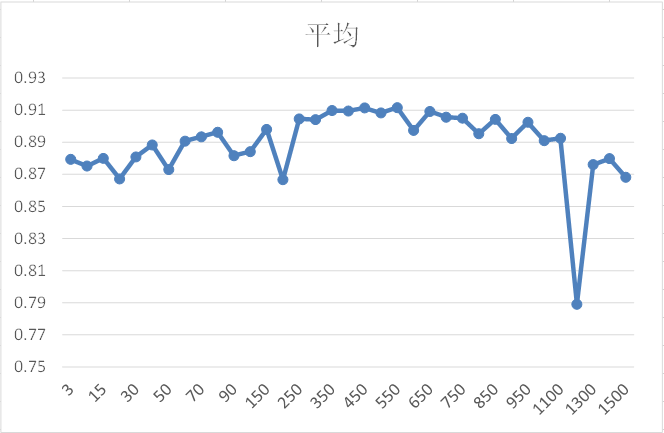
\includegraphics[width=0.9\textwidth]{实验数据1.png}
  \caption{实验数据的平均值}
  \label{fig:shuju1}
\end{figure}

\begin{figure}[!htb]
  \centering
  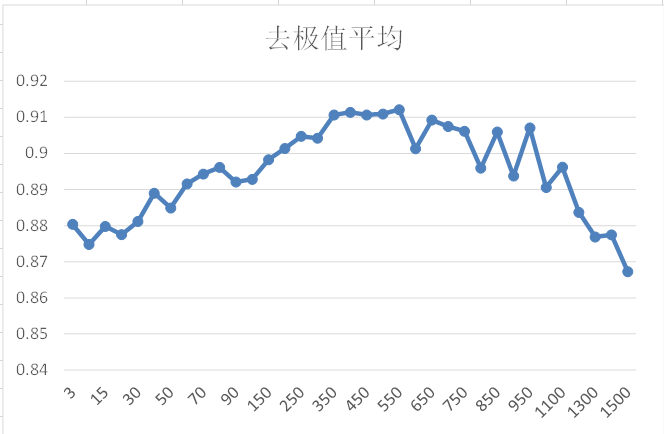
\includegraphics[width=0.9\textwidth]{实验数据1-去极值.png}
  \caption{实验数据的去极值平均值}
  \label{fig:shuju1qujizhi}
\end{figure}

我使用地形分支节点数为550训练出来的模型在测试集上进行预测,并获取了训练集和验证集的正确率和损失值随着迭代次数变化的图,如图\ref{fig:train-acc1}和\ref{fig:train-loss1}
\begin{figure}[!htb]
  \centering
  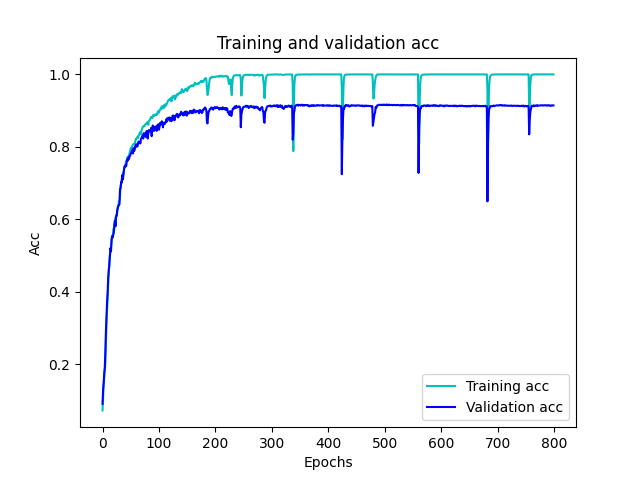
\includegraphics[width=0.9\textwidth]{save_acc2.png}
  \caption{地形分支节点数为550的训练集和验证集的实验精度}
  \label{fig:train-acc1}
\end{figure}
\begin{figure}[!htb]
  \centering
  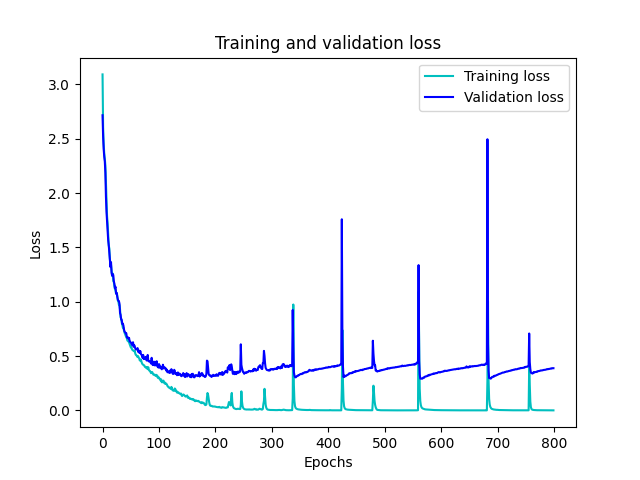
\includegraphics[width=0.9\textwidth]{save_loss2.png}
  \caption{地形分支节点数为550的训练集和验证集的损失值}
  \label{fig:train-loss1}
\end{figure}


\subsection{方案二:无全连接层+多输出}
在两个分支进行合并后直接送入$softmax$分类器进行分类,分类的输出方式为多输出。即输出7个一级地物标签和20个二级地物标签。本实验二的地形分支的节点数选取
方法一中所得到的550.本实验需要调节的超参数为一级地物标签的损失值和二级地物标签的损失值的加权系数。二级地物的系数固定为1,一级地物的系数的所选取的范围为0-1(一步为0.1)和1-10(一步为1)。

每个加权系数运行5次,最后取平均值和去极值平均值。部分加权系数的5次运行所得到的验证集结果如表\ref{tab:table2}所示。
各个加权系数5次运行的正确率平均值可见图\ref{fig:shiyanshu2junzhi},去极值平均的结果可见图\ref{fig:shiyanshu2qujizhi}.
由图\ref{fig:shiyanshu2junzhi}和\ref{fig:shiyanshu2qujizhi}可知,一级地物标签的加权系数为0.3时,实验的验证集正确率最高,故选定一级地物标签的损失值加权系数为0.3.

% Table generated by Excel2LaTeX from sheet 'Sheet1'
\begin{table}[htbp]
  \centering
  \caption{部分加权系数的5次运行结果}
    \begin{tabular}{|c|c|c|c|c|c|}
    \toprule
          & \textbf{0.1} & \textbf{0.2} & \textbf{0.3} & \textbf{0.4} & \textbf{0.5} \\
    \midrule
    \textbf{1} & 0.911 & 0.9023 & 0.9113 & 0.91  & 0.8985 \\
    \midrule
    \textbf{2} & 0.9113 & 0.9138 & 0.9135 & 0.9058 & 0.9111 \\
    \midrule
    \textbf{3} & 0.9113 & 0.9087 & 0.9118 & 0.916 & 0.9077 \\
    \midrule
    \textbf{4} & 0.9131 & 0.9136 & 0.9125 & 0.8999 & 0.8815 \\
    \midrule
    \textbf{5} & 0.9131 & 0.9112 & 0.914 & 0.914 & 0.9124 \\
    \midrule
    平均    & \cellcolor[rgb]{ 1,  0,  0}0.91196 & 0.90992 & \cellcolor[rgb]{ .753,  0,  0}0.91262 & 0.90914 & 0.90224 \\
    \midrule
    去极值平均 & \cellcolor[rgb]{ 1,  0,  0}0.9119 & 0.911167 & \cellcolor[rgb]{ .753,  0,  0}0.9126 & 0.909933 & 0.905767 \\
    \bottomrule
    \end{tabular}%
  \label{tab:table2}%
\end{table}%

\begin{figure}[!htb]
  \centering
  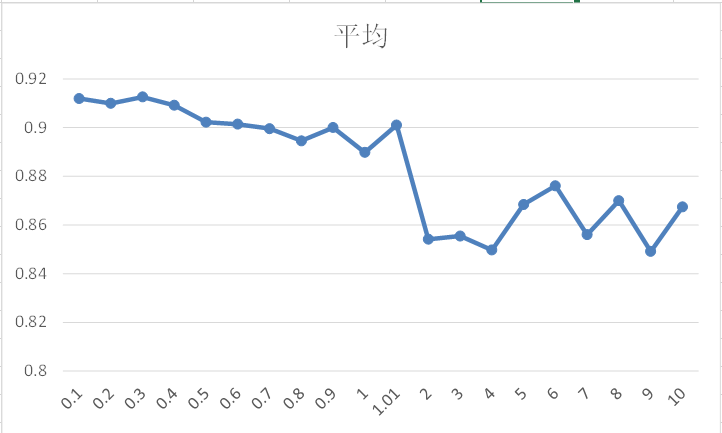
\includegraphics[width=0.9\textwidth]{实验数据2-均值.png}
  \caption{各个加权系数5次运行的正确率平均值}
  \label{fig:shiyanshu2junzhi}
\end{figure}

\begin{figure}[!htb]
  \centering
  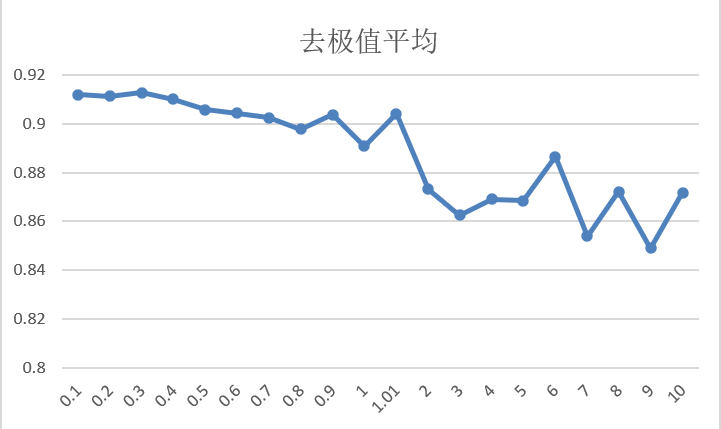
\includegraphics[width=0.9\textwidth]{图片1.png}
  \caption{各个加权系数5次运行的正确率去极值平均值}
  \label{fig:shiyanshu2qujizhi}
\end{figure}

我使用一级地物加权系数为0.3训练得到的模型对测试集进行预测,并获取了其在训练集和验证集上的正确率和损失值随着迭代次数变化的图,其中验证集的变化如图\ref{fig:val-acc2}和\ref{fig:val-loss2}所示

\begin{figure}[!htb]
  \centering
  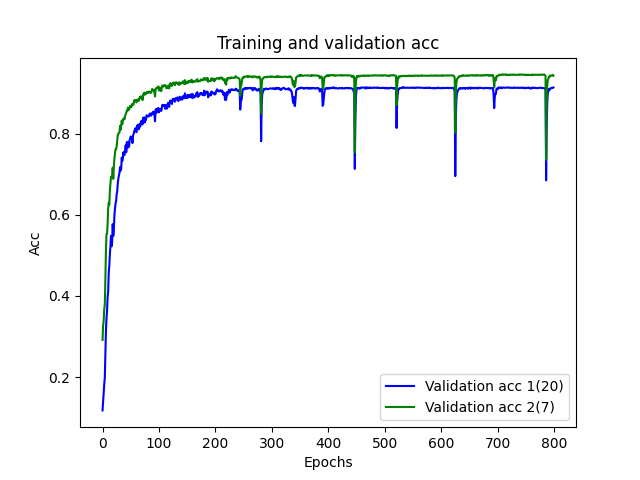
\includegraphics[width=0.9\textwidth]{save_Va_acc-1-3.0.png}
  \caption{一级地物的加权系数为0.3的验证集正确率}
  \label{fig:val-acc2}
\end{figure}

\begin{figure}[!htb]
  \centering
  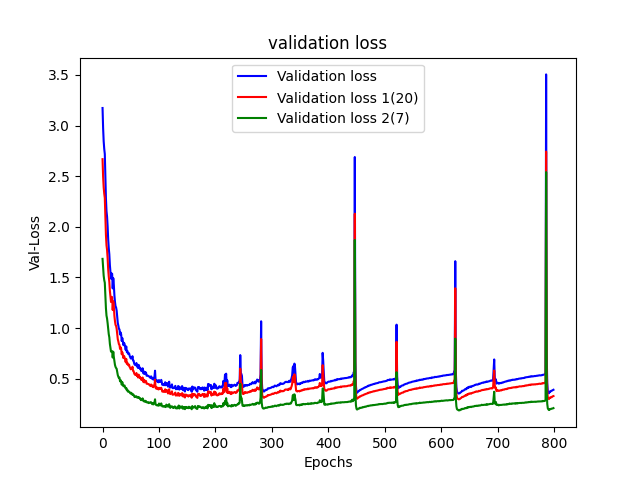
\includegraphics[width=0.9\textwidth]{save_Va_loss-1-3.0.png}
  \caption{一级地物的加权系数为0.3的验证集损失值}
  \label{fig:val-loss2}
\end{figure}


\subsection{方案三:一个全连接层+单输出}
本实验在两个分支进行合并后再输入到一层全连接层,然后再送入$softmax$分类器进行分类,分类的输出方式为单输出,即只输出20个二级地物标签的类别。本实验没有需要调节的超参数,地形分支节点数为方法一中所选取的550。
全连接层的节点数为空间-光谱分支的节点数与地形分支的节点数的加和,即$1500+550=2050$.

使用该模型对测试集结果进行预测,并获取到其在训练集与验证集上的精度与损失值随着迭代次数的变化情况的图,如图\ref{fig:train-acc3}和\ref{fig:train-loss3}所示。

\begin{figure}[!htb]
  \centering
  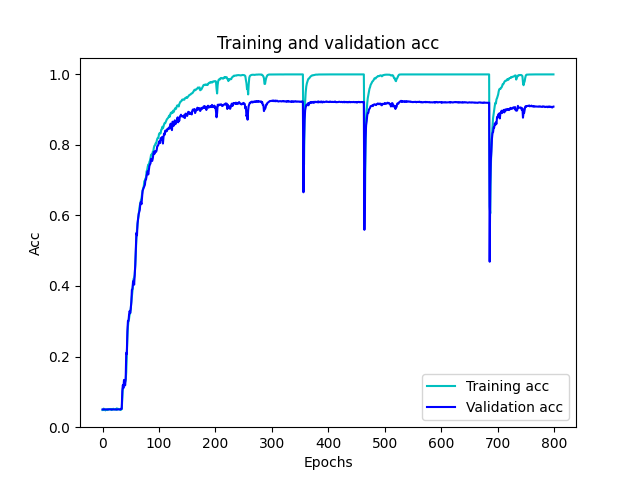
\includegraphics[width=0.9\textwidth]{save_acc3.png}
  \caption{方法三在训练集与验证集上的精度变化}
  \label{fig:train-acc3}
\end{figure}

\begin{figure}[!htb]
  \centering
  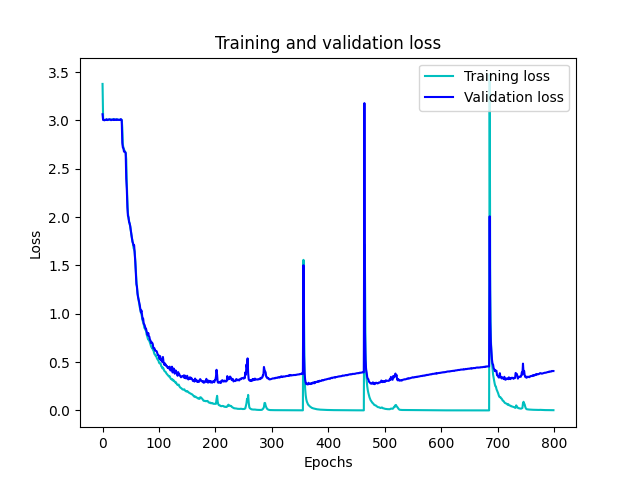
\includegraphics[width=0.9\textwidth]{save_loss3.png}
  \caption{方法三在训练集与验证集上的损失值变化}
  \label{fig:train-loss3}
\end{figure}

\subsection{方法四:一个全连接层+多输出}
本实验在两个分支进行合并后再输入到一层全连接层,然后再送入$softmax$分类器进行分类,分类的输出方式为多输出,即输出7个一级地物标签和20个二级地物标签。本实验四的地形分支的节点数为方法一中所选取的550,一级地物的损失加权系数为方法二中所选取的0.3.全连接层的节点数为空间-光谱分支的节点数与地形分支的节点数的加和,即$1500+550=2050$.

使用该模型对测试集结果进行预测,并获取到其在训练集与验证集上的精度与损失值随着迭代次数的变化情况的图,验证集精度和损失变化如图\ref{fig:val-acc4}和\ref{fig:val-loss4}所示。

\begin{figure}[!htb]
  \centering
  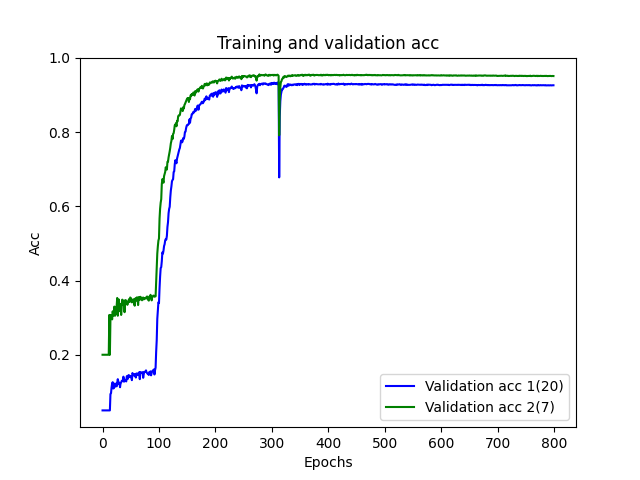
\includegraphics[width=0.9\textwidth]{save_Va_acc-5-3.0.png}
  \caption{方法四在验证集上的精度变化}
  \label{fig:val-acc4}
\end{figure}

\begin{figure}[!htb]
  \centering
  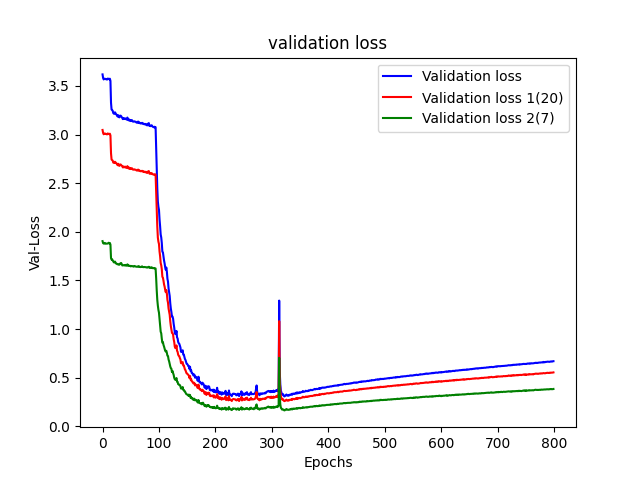
\includegraphics[width=0.9\textwidth]{save_Va_loss-5-3.0.png}
  \caption{方法四在验证集上的损失值变化}
  \label{fig:val-loss4}
\end{figure}


\subsection{方法对比}
我们根据上述四种方法确定了地形分支的节点数为550,在多输出方面,一级地物损失值的及加权系数为0.3.接着,我们将训练好的四种方法的模型
应用到测试集上进行对比,对比使用五组测试集,并求得平均进行比较,实验结果如表\ref{tab:table3}所示。
% Table generated by Excel2LaTeX from sheet 'Sheet1'
% Table generated by Excel2LaTeX from sheet 'Sheet1'
\begin{table}[htbp]
  \centering
  \caption{方法对比}
    \begin{tabular}{|c|c|c|c|c|c|c|}
    \toprule
          & 测试集1  & 测试集2  & 测试集3  & 测试集4  & 测试集5  & 平均值 \\
    \midrule
    方法1   & 0.9129 & 0.9181 & 0.9172 & 0.9203 & 0.919 & \cellcolor[rgb]{ 1,  .486,  .502}0.9175 \\
    \midrule
    方法2   & 0.9139 & 0.9141 & 0.919 & 0.9162 & 0.9134 & \cellcolor[rgb]{ 1,  .8,  .8}0.91532 \\
    \midrule
    方法3   & 0.9333 & 0.9296 & 0.9357 & 0.9355 & 0.9346 & \cellcolor[rgb]{ .753,  0,  0}0.93374 \\
    \midrule
    方法4   & 0.9259 & 0.9251 & 0.9274 & 0.9287 & 0.9267 & \cellcolor[rgb]{ 1,  0,  0}0.92676 \\
    \bottomrule
    \end{tabular}%
  \label{tab:table3}%
\end{table}%

由表\ref{tab:table3}可以看出,方法3一个全连接层加单输出的方式在五组测试集上结果最好
实验平均值达到了0.93374.其次是方法4一个全连接层加多输出的方式,达到了0.92676.由此可见,在原来的模型上加上一个全连接层,可使当前的分类结果更好。
对于多输出模型的精度小于单输出模型精度的,可能是由多输出模型在训练集上过拟合导致的。





\section{实验二-SVM}
\subsection{固定参数}
我们在本实验中使用的固定参数与实验一相同,并且在实验一的基础上,我们得到了地形分支的节点数为550,并且在多输出方面,一级地物的损失值加权系数设为0.3。

\subsection{模型选择}
我们使用由方法一得到的四个模型来获取深度特征,并将其输入到$SVM$分类器中进行分类。
选取在测试集上分类效果最好的模型来对$SVM$分类器进行调整参数,实验结果如表\ref{tab:table4}所示。

% Table generated by Excel2LaTeX from sheet 'Sheet1'
\begin{table}[htbp]
  \centering
  \caption{模型选择}
    \begin{tabular}{|c|r|r|}
    \toprule
          & \multicolumn{1}{c|}{\textbf{无}} & \multicolumn{1}{c|}{\textbf{SVM}} \\
    \midrule
    \textbf{方法1} & 0.9129 & 0.9491 \\
    \midrule
    \textbf{方法2} & 0.9139 & \cellcolor[rgb]{ .753,  0,  0}0.9497 \\
    \midrule
    \textbf{方法3} & \cellcolor[rgb]{ .753,  0,  0}0.9333 & 0.9378 \\
    \midrule
    \textbf{方法4} & 0.9259 & 0.9324 \\
    \bottomrule
    \end{tabular}%
  \label{tab:table4}%
\end{table}%

由表\ref{tab:table4}可以看出,方法2的模型所得到的结果最好,故选取方法二的模型作为SVM的超参数调整模型。

\subsection{参数调整}
对于 DBN-SVM 模型,对 cost 和 gamma 进行了优化。总共使用了 30种组合,即cost选取6个值(0.5,2,8,32,128,512),gamma选取5个值($2^{-11}$,$2^{-9}$,$2^{-7}$,$2^{-5}$,$2^{-3}$)。
我们获得了该30个组合在验证集上的结果,
由表\ref{tab:table5}可以看出,gamma值可以确定选取$2^{-5}$,对于cost值,因为当值为2,8,32,128,512时,其精度相差不大,故选取该五个值均在测试集上获取结果。

% Table generated by Excel2LaTeX from sheet 'Sheet1'
\begin{table}[htbp]
  \centering
  \caption{30个组合在验证集上的精度}
    \begin{tabular}{|c|c|c|c|c|c|}
    \toprule
    \diagbox{cost}{gamma} & \textbf{0.00049} & \textbf{0.00195} & \textbf{0.00781} & \textbf{0.03125} & \textbf{0.125} \\
    \midrule
    \textbf{0.5} & 0.8952 & 0.9146 & 0.9289 & 0.9468 & 0.7859 \\
    \midrule
    \textbf{2} & 0.9133 & 0.9221 & 0.9347 & \cellcolor[rgb]{ .753,  0,  0}0.95 & 0.882 \\
    \midrule
    \textbf{8} & 0.9179 & 0.9237 & 0.9331 & \cellcolor[rgb]{ 1,  .6,  .8}0.9497 & 0.8821 \\
    \midrule
    \textbf{32} & 0.9199 & 0.923 & 0.9319 & \cellcolor[rgb]{ 1,  0,  0}0.9498 & 0.882 \\
    \midrule
    \textbf{128} & 0.92  & 0.9223 & 0.932 & \cellcolor[rgb]{ 1,  .6,  .8}0.9497 & 0.882 \\
    \midrule
    \textbf{512} & 0.9194 & 0.9221 & 0.9318 & \cellcolor[rgb]{ 1,  .6,  .8}0.9497 & 0.882 \\
    \bottomrule
    \end{tabular}%
  \label{tab:table5}%
\end{table}%


在\ref{tab:table6}中,我们可以看到在测试集上精度最好的的cost值是8,其所得到的精度为0.95.由此,我们得到了SVM的最佳超参数组合为cost=8,gamma=$2^{-5}$,使得最后的分类精度达到了$95\%$.

% Table generated by Excel2LaTeX from sheet 'Sheet1'
% Table generated by Excel2LaTeX from sheet 'Sheet1'
\begin{table}[htbp]
  \centering
  \caption{5个cost参数在测试集上的精度}
    \begin{tabular}{|c|r|}
    \toprule
    \diagbox{cost}{gamma} & \multicolumn{1}{c|}{\textbf{0.03125}} \\
    \midrule
    \textbf{2} & \cellcolor[rgb]{ .988,  .835,  .706}0.9497 \\
    \midrule
    \textbf{8} & \cellcolor[rgb]{ 1,  1,  0}\textcolor[rgb]{ 1,  0,  0}{0.95} \\
    \midrule
    \textbf{32} & \cellcolor[rgb]{ .769,  .843,  .608}0.9499 \\
    \midrule
    \textbf{128} & \cellcolor[rgb]{ .769,  .843,  .608}0.9499 \\
    \midrule
    \textbf{512} & \cellcolor[rgb]{ .769,  .843,  .608}0.9499 \\
    \bottomrule
    \end{tabular}%
  \label{tab:table6}%
\end{table}%

\subsection{实验对比}
和实验一的对比相同,我们选取方法一到方法四的模型并与SVM分类器结合来预测测试集分类结果。其中SVM分类器的超参数选择前面所得到的最优参数组合cost=8,gamma=$2^{-5}$.
同样的,使用5组测试集,并对最后求得的精度进行平均来对比,实验结果如表\ref{tab:table7}所示。


% Table generated by Excel2LaTeX from sheet 'Sheet1'
\begin{table}[htbp]
  \centering
  \caption{模型对比}
    \begin{tabular}{|c|c|c|c|c|c|c|}
    \toprule
          & 测试集1  & 测试集2  & 测试集3  & 测试集4  & 测试集5  & 平均值 \\
    \midrule
    方法1+svm & 0.9491 & 0.9533 & 0.9547 & 0.9573 & 0.9549 & \cellcolor[rgb]{ .753,  0,  0}0.95386 \\
    \midrule
    方法2+svm & 0.95  & 0.9476 & 0.9527 & 0.9538 & 0.9515 & \cellcolor[rgb]{ 1,  0,  0}0.95112 \\
    \midrule
    方法3+svm & 0.9378 & 0.9367 & 0.9419 & 0.9409 & 0.939 & \cellcolor[rgb]{ 1,  .486,  .502}0.93926 \\
    \midrule
    方法4+svm & 0.9324 & 0.9302 & 0.9347 & 0.9359 & 0.9319 & \cellcolor[rgb]{ 1,  .8,  .8}0.93302 \\
    \bottomrule
    \end{tabular}%
  \label{tab:table7}%
\end{table}%

由\ref{tab:table7}可以看出,方法一的模型加上SVM可以使得分类结果最好,其结果为$95.386\%$,其次方法所得到的结果依次递减。
其中可能的原因为,和$softmax$不同,不加全连接层所得到的深度特征,能够使得SVM分类器得到更好的结果。

\section{实验三-RF}
实验中的方法一到方法四的模型与SVM中的模型相同,让后将其送入RF分类器中进行分类。我们使用五组测试集,最后取平均的方式来评价各个模型。四个模型在五组测试集上的结果如表\ref{tab:table8}所示。


% Table generated by Excel2LaTeX from sheet 'Sheet1'
\begin{table}[htbp]
  \centering
  \caption{RF分类器在五组测试集上的精度}
    \begin{tabular}{|c|c|c|c|c|c|c|}
    \toprule
          & 测试集1  & 测试集2  & 测试集3  & 测试集4  & 测试集5  & 平均值 \\
    \midrule
    方法1+RF & 0.9189 & 0.9242 & 0.9248 & 0.9255 & 0.9242 & \cellcolor[rgb]{ 1,  0,  0}0.92352 \\
    \midrule
    方法2+RF & 0.9162 & 0.9189 & 0.9221 & 0.9213 & 0.9177 & \cellcolor[rgb]{ 1,  .486,  .502}0.91924 \\
    \midrule
    方法3+RF & 0.9244 & 0.9262 & 0.9305 & 0.9298 & 0.9287 & \cellcolor[rgb]{ .753,  0,  0}0.92792 \\
    \midrule
    方法4+RF & 0.9131 & 0.9177 & 0.9215 & 0.9173 & 0.917 & \cellcolor[rgb]{ 1,  .8,  .8}0.91732 \\
    \bottomrule
    \end{tabular}%
  \label{tab:table8}%
\end{table}%


\end{document}
